%
% $Id: filter_design.tex 14 2014-02-04 22:36:30Z nicb $
%
% cap.12
%
\svnInfo $Id: filter_design.tex 14 2014-02-04 22:36:30Z nicb $

\section{Introduzione alla progettazione di filtri FIR\label{sec: filter design introduction}}
%
% tecniche di design: ottimizzazione iterativa
%                   forme chiuse
%

Il problema sostanziale nel progettare i filtri \`e quello di trovare i giusti
coefficienti per raggiungere la migliore approssimazione alla ``risposta ideale''
che si desidera ottenere. In linea generale, la ``risposta ideale'' non \`e
ottenibile direttamente perch\'e si tratta di una funzione discontinua (che
non \`e realizzabile con un polinomio. Il problema \`e rappresentato in
fig.\vref{fig:ideal vs real}.
\begin{figure}[htbp]
	\begin{center}
		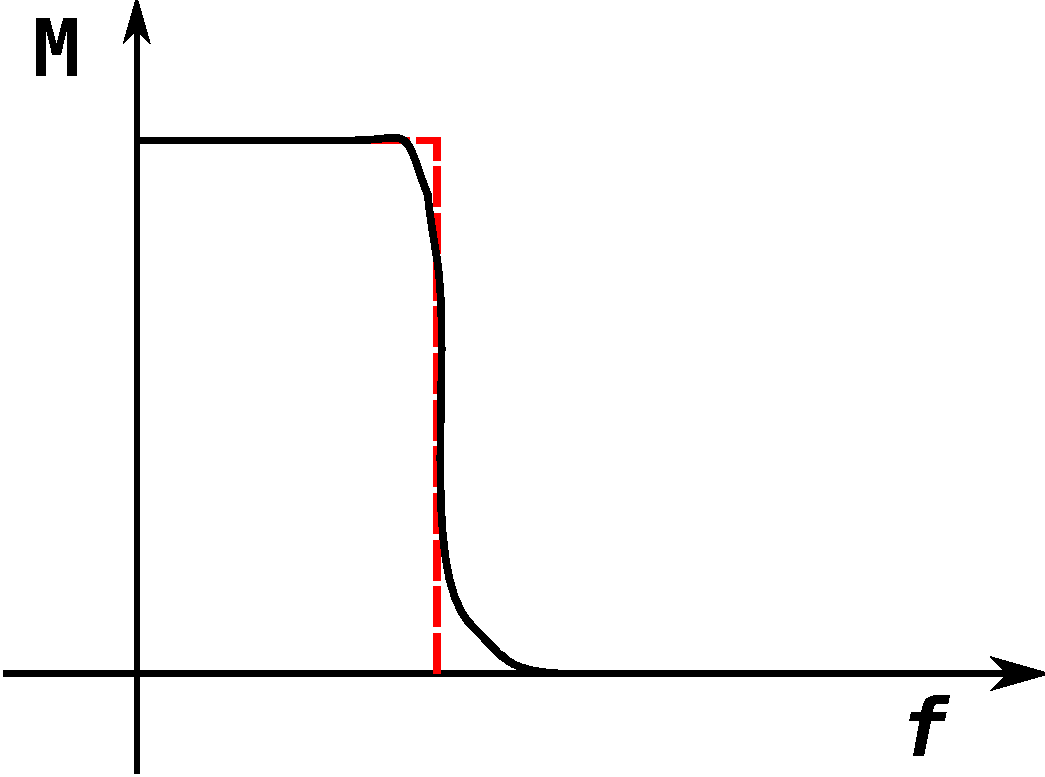
\includegraphics[width=0.75\textwidth]{\imagedir/ideal_vs_real}
		\caption{La risposta ideale di un filtro (in rosso) e la sua risposta reale\label{fig:ideal vs real}}
	\end{center}
\end{figure}

Ci sono varie soluzioni per ottenere questi coefficienti, e queste soluzioni
si applicano meglio a certi tipi di filtri che ad altri.
In alcuni casi \`e possibile (o necessario) trovare delle ``forme chiuse''
(vale a dire delle equazioni matematiche finite) per individuare i
coefficienti, mentre in altri casi \`e possibile trovarli attraverso una
``ottimizzazione iterativa'' (vale a dire ottenendo prima una approssimazione
mediocre per poi migliorarla a discrezione).

I coefficienti dei filtri FIR si trovano pi\`u facilmente attraverso
quest'ultima tecnica (ottimizzazione iterativa).

%
% ordine del filtro e simmetria dei coefficienti (0, N-1 per N coefficienti, N-1 ordine)
%

Ricordiamo che la forma dei filtri FIR \`e specificata da un'equazione del
tipo:

\begin{equation}
	y_t = a_0 x_t + a_1 x_{t-1} + a_2 x_{t-2} + \dots + a_{n-1} x_{t-(n-1)}
\end{equation}

Il primo coefficiente \`e il coefficiente $0$, quindi l'ultimo coefficiente di
un filtro di lunghezza $n$ \`e $n-1$. La sua funzione di trasferimento \`e

\begin{equation}
	H(z) = a_0 + a_1 z^{-1} + a_2 z^{-2} + \dots + a_{n-1} z^{-(n-1)}
\end{equation}

Considerando che la risposta $y_t$ deve essere una risposta reale, possiamo
semplificare la nostra progettazione utilizzando un numero pari di
coefficienti. Questi coefficienti distribuiranno gli zeri sul piano zeta in
posizioni complesse--coniugate ed il risultato sar\`a quindi reale.
Il problema \`e che abbiamo un coefficiente $0$, e che quindi se usiamo filtri
di lunghezza pari avremo una asimmetria intorno all'asse dei numeri reali.
Dobbiamo quindi utilizzare una lunghezza \emph{dispari} per ottenere un numero
\emph{pari} di coefficienti simmetrici (e un coefficiente direttamente
sull'asse reale -- che quindi sar\`a un numero reale).

Ad esempio, se usiamo un filtro di lunghezza 5, avremo la funzione di
trasferimento

\begin{equation}\label{eqn: fir order five}
		H(z) = a_0 + a_1 z^{-1} + a_2 z^{-2} + a_3 z^{-3} + a_4 z^{-4}
\end{equation}

Il trucco standard \`e quello di mettere a fattore una potenza di $z$
corrispondente al \emph{ritardo medio} del nostro filtro. Nel caso
dell'equazione \ref{eqn: fir order five} il ritardo medio sar\`a $z^{-2}$.
L'equazione viene cos\`i riscritta

\begin{equation}\label{eqn: fir order five rewritten}
	H(z) = z^{-2} \left [ a_0 z^{2} + a_1 z + a_2 + a_3 z^{-1} + a_4 z^{-2} \right ]
\end{equation}

La risposta in frequenza corrispondente viene ottenuta, come sempre,
sostituendo $z = e^{i \omega}$.

\begin{equation}\label{eqn: fir order five freq response}
	H(\omega) = e^{-i2\omega} \left [ a_0 e^{i2\omega} + a_1 e^{i\omega} + a_2 + a_3 e^{-i\omega} + a_4 e^{-i2\omega} \right ]
\end{equation}

Abbiamo visto che coefficienti simmetrici producono una risposta in fase
lineare. Daremo quindi per scontato che $a_0 = a_4$ e $a_1 = a_3$.
Ma 

\begin{equation}
	a_0 ( e^{i 2 \omega} + e^{-i 2 \omega} ) = 2 a_0 cos(2 \omega)
\end{equation}

e

\begin{equation}
	a_1 ( e^{i \omega} + e^{-i \omega} ) = 2 a_1 cos(\omega)
\end{equation}

Quindi:

\begin{equation}\label{eqn: fir order five freq response rewritten}
	H(\omega) = e^{-i2\omega} \left [ a_2 + 2 a_1 cos \omega + 2 a_0 cos (2 \omega) \right ]
\end{equation}

Come si pu\`o notare, la parte fra parentesi quadre \`e \emph{reale}, e il
fattore complesso che la moltiplica altro non \`e che un ritardo
``complessivo'' di due campioni. Questo fattore non influisce sulla
magnitudine del filtro, perch\'e il modulo di $e^{-i 2 \omega}$ \`e $1$.

Per semplificare ulteriormente, possiamo utilizzare dei coefficienti $c_i$ in
ordine ascendente, riscrivendo cos\`i l'equazione \ref{eqn: fir order five freq response rewritten} come:

\begin{equation}\label{eqn: fir order five freq response rewritten 2}
  \hat{H}(\omega) = e^{i2\omega} H(\omega) = c_0 + c_1 cos \omega + c_2 cos (2 \omega)
\end{equation}

dove $c_0 = a_2$, $c_1 = 2 a_1$ e $c_2 = 2 a_0$. Il ritardo lo abbiamo
spostato a sinistra dell'equazione (dove in realt\`a \`e un anticipo piuttosto
che un ritardo).

La nuova risposta in frequenza $\hat{H}(\omega)$ incorpora quindi il ritardo
generale ed \`e esclusivamente reale.
Per semplificarci la vita ulteriormente, diamo per scontato che la lunghezza
del filtro sia sempre un intero dispari.
\`E facile notare che la forma generale dell'eq.\ref{eqn: fir order five freq response rewritten}
\`e

\begin{equation}\label{eqn: fir rewritten general form}
  \hat{H}(\omega) = e^{im\omega} H(\omega) = c_0 + c_1 cos \omega + c_2 cos (2 \omega) + \dots + c_m cos (m \omega)
\end{equation}

dove $m = 1/2 (n - 1)$.
Dal momento che contiamo sempre a partire da $0$, ci saranno $m + 1 = 1/2 (n + 1)$ coefficienti $c$.
Dato che i coefficienti $a$ sono simmetrici, $m + 1$ saranno i coefficienti
con i quali avremo a che fare.

Ultima cosa: dato che a noi interessa soprattutto la magnitudine della
risposta in frequenza, considereremo quindi la parte destra dell'equazione
\ref{eqn: fir rewritten general form} senza il ritardo.
Questa parte sar\`a costituita da valori reali sia positivi che negativi.
Volendo, possiamo interpretare la magnitudine negativa come un shift di fase di $\pi$
radianti.

Riassumendo: quando disegniamo un filtro FIR, diamo per scontato che questi
filtri abbiano un numero dispari di termini ($n$)
i cui coefficienti siano simmetrici intorno al termine centrale.
La risposta in frequenza \`e quindi determinata dalla serie (solo di valori
reali) dei coseni dell'eq.\ref{eqn: fir rewritten general form} con $m = 1/2 ( n + 1 ) $
incognite $c_i$.
Il problema della progettazione del filtro si riduce cos\`i alla scelta di
questi coefficienti $c_i$ in modo da soddisfare le specifiche date.

%
% aggiungere qui la definizione di passband, stopband e boundaries
%

La chiave della soluzione \`e legata al fatto che la risposta in frequenza
della serie dei coseni in eq.\ref{eqn: fir rewritten general form} \`e una
funzione \emph{lineare} con coefficienti sconosciuti.
Facciamo un esempio volutamente molto semplice per illustrare l'idea.
Supponiamo di voler progettare un filtro di lunghezza $3$ -- nel quale dovremo
scegliere appunto due soli coefficienti.
Potremmo dare le specifiche seguenti:

\begin{compactenum}

	\item nella parte \emph{passband}, il confine superiore della funzione non
					deve superare il valore $1.05$, ossia:

					\begin{equation}
						\hat{H} (\omega) = c_0 + c_1 cos \omega \leq 1.05
					\end{equation}

	
	\item nella parte \emph{passband}, il confine inferiore della funzione non
					non deve essere meno di $0.95$, ossia:

					\begin{equation}
						\hat{H} (\omega) = c_0 + c_1 cos \omega \geq 0.95
					\end{equation}

	\item e cos\`i via.

\end{compactenum}

Si mettono insieme tante ``restrizioni'' di questo tipo suddividendo la
funzione in tanti punti e poi si cercano i coefficienti $c_i$ che
soddisfino simultaneamente tutti questi punti. Se, ad esempio, suddividiamo la
parte \emph{passband} in 500 punti e la parte \emph{stopband} in altri 500
punti, avremo 1000 ``restrizioni'' da rispettare simultaneamente.
La soluzione sembra molto difficile, ma in realt\`a la matematica degli anni '40 
ha trovato degli algoritmi (detti di \emph{programmazione lineare})
per risolvere questo tipo di problemi.
Questo tipo di problemi si chiama \emph{minimax} perch\'e vogliamo
\emph{massimizzare la distanza minima} per ogni ``restrizione''.

A questo punto, tenendo conto del fatto che i coefficienti che si stanno
cercando sono quelli di una serie di coseni, possiamo utilizzare una serie di
Fourier di soli coseni con le ampiezze che soddisfino le restrizioni poste. I
coefficienti della serie dovranno essere opportunamente ``finestrati'' per
evitare il fenomeno del \emph{ripple} nella parte \emph{passband} e nella
parte \emph{band--reject}.
La lunghezza del filtro sar\`a basata sulle restrizioni poste sulla larghezza
di banda della transizione.

%
% scelta dell'ordine del filtro
%
